

\documentclass[10pt,journal,cspaper,compsoc,onecolumn]{IEEEtran}

\usepackage{enumerate}
\usepackage{cite}
\usepackage{amsmath}
\interdisplaylinepenalty=2500
\usepackage{algorithm}
\usepackage{algorithmic}
\usepackage{graphicx}
\usepackage{multirow}
\usepackage{subfigure}
\usepackage{amssymb}
\usepackage[normalem]{ulem}
\usepackage{color}
\usepackage{ulem}
\usepackage{booktabs}
\allowdisplaybreaks[4]
\hyphenation{op-tical net-works semi-conduc-tor}


\begin{document}
\large{\textbf{Appendix B: Experimental Results}}

F-, F2-, and T-measure results for each program are displayed using boxplots in Figures \ref{fig:appendixFmeasure} to \ref{fig:appendixTmeasure}, where $DRT_i$ $(i = 1,2, \ldots, 13)$ denotes the DRT with different values of $\varepsilon$, as described in Section 4.4.3.

\begin{figure*}[h]
	\centering
    \subfigure[ACMS] {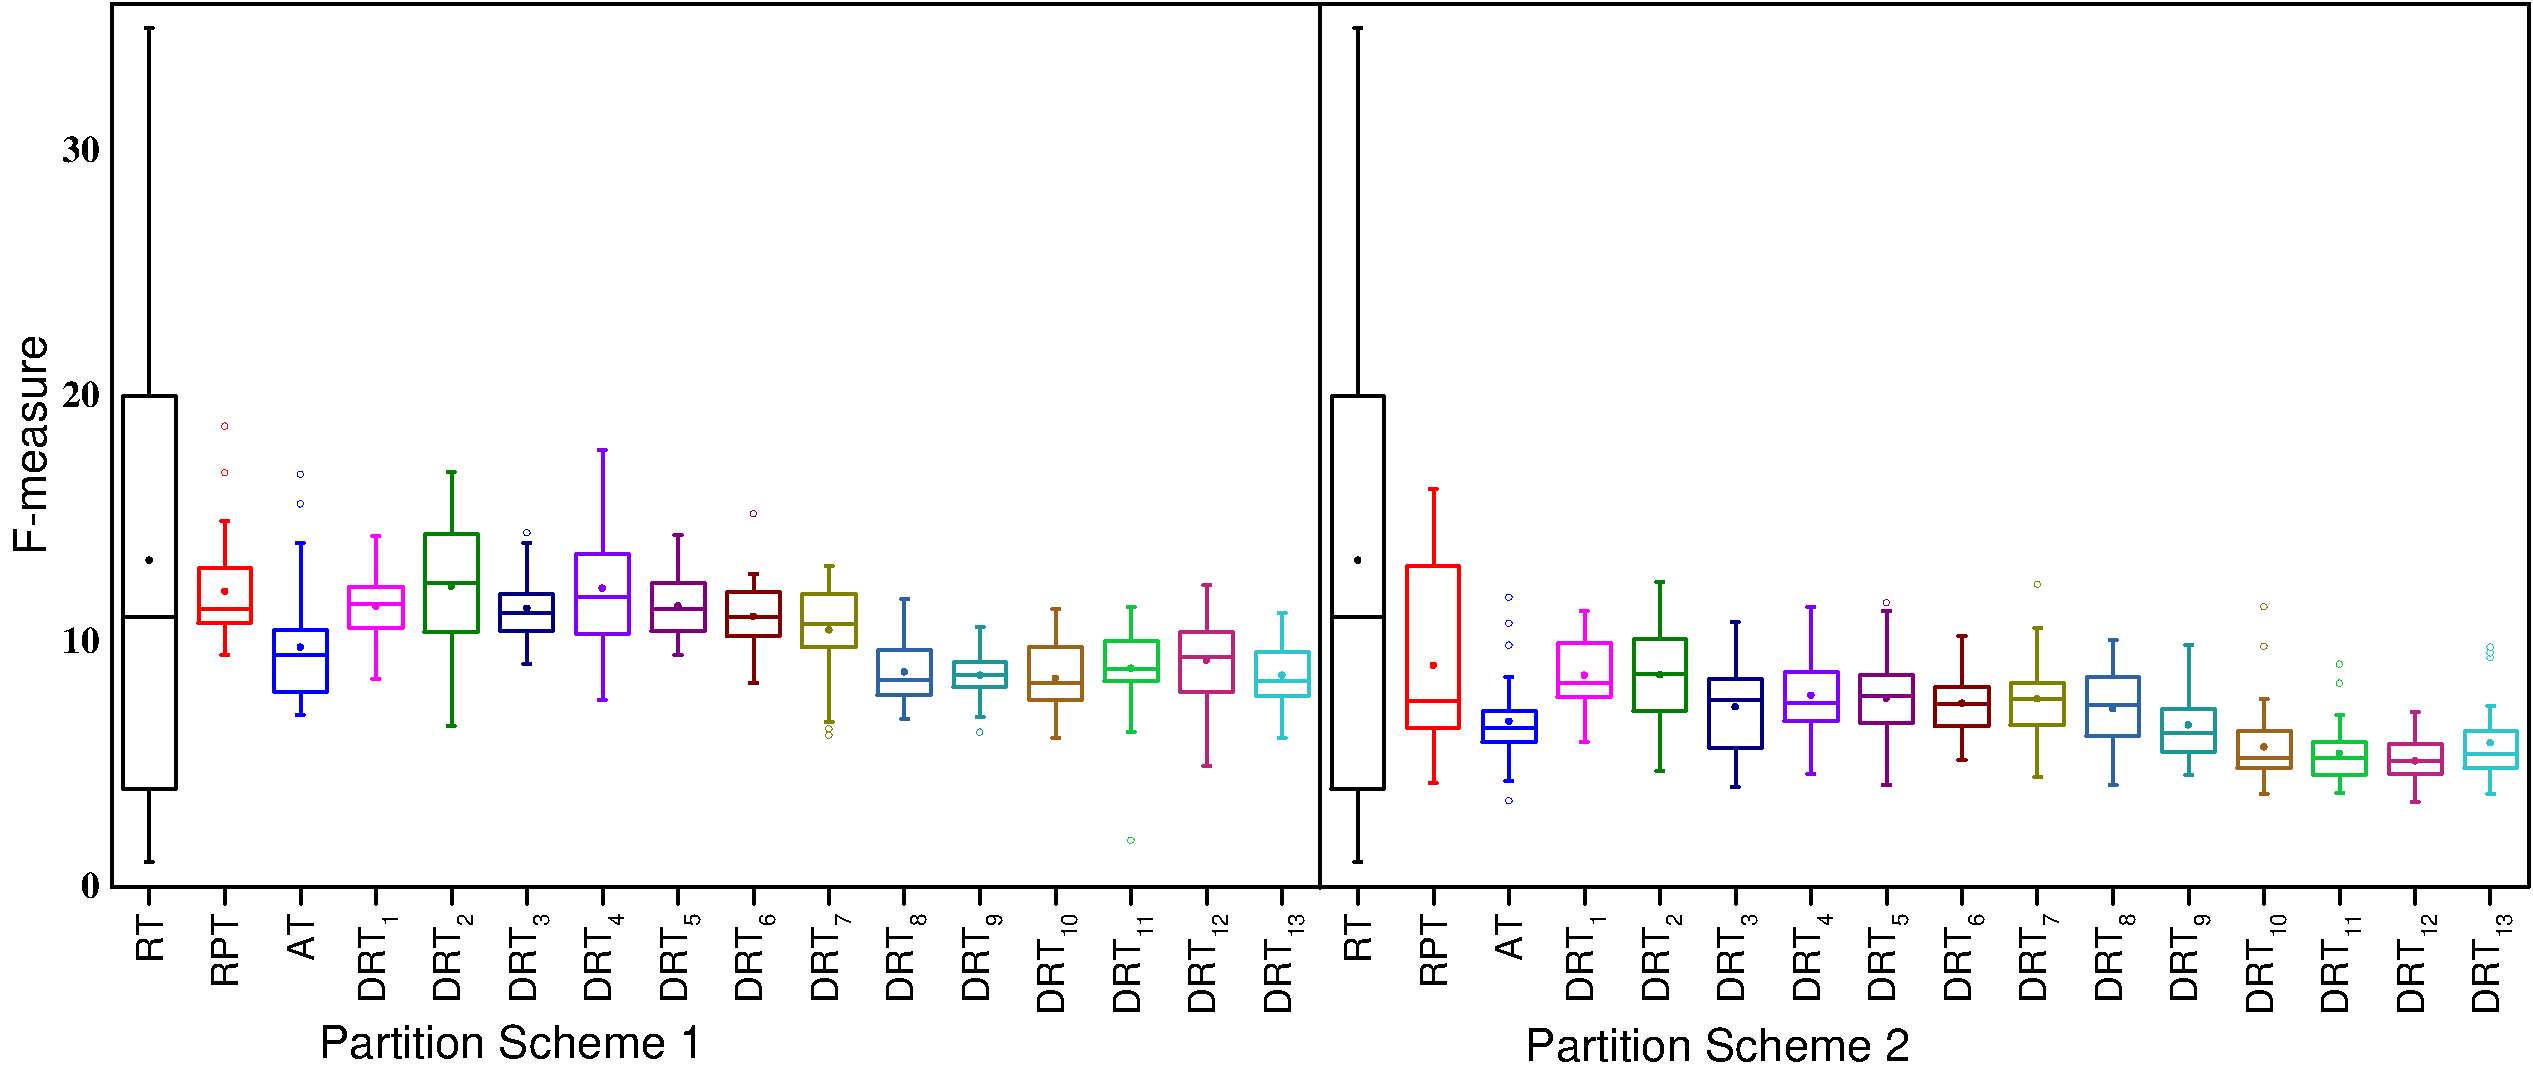
\includegraphics[width=0.9\textwidth,height=6.25cm]{fig/drtresultbox/aviaresultf.pdf}}
	\subfigure[CUBS] {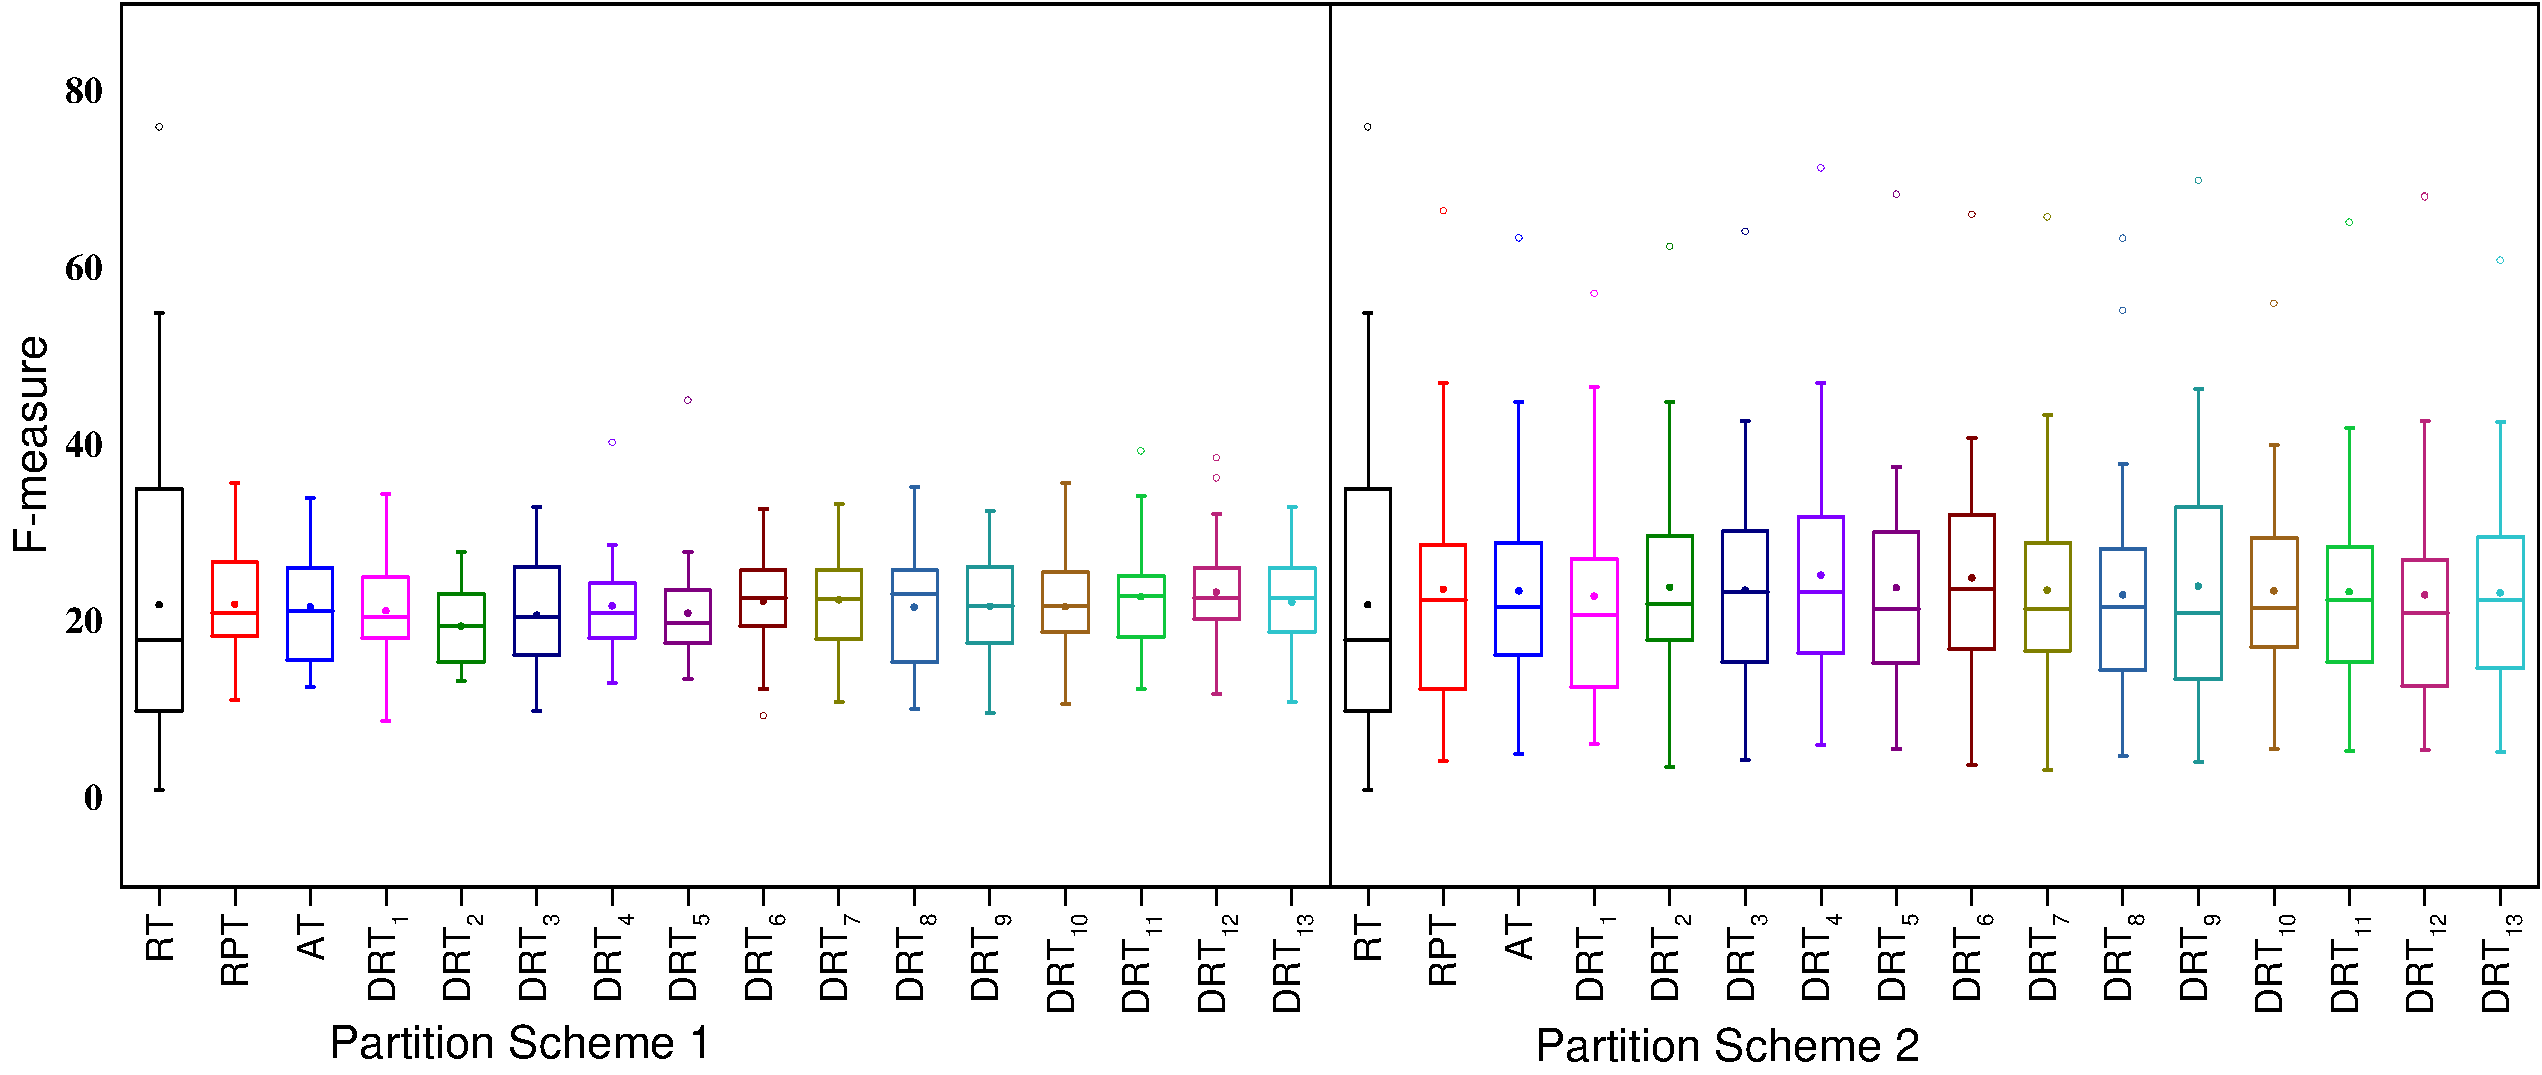
\includegraphics[width=0.9\textwidth,height=6.2cm]{fig/drtresultbox/chinaresultf.pdf}}
	\subfigure[PBS] {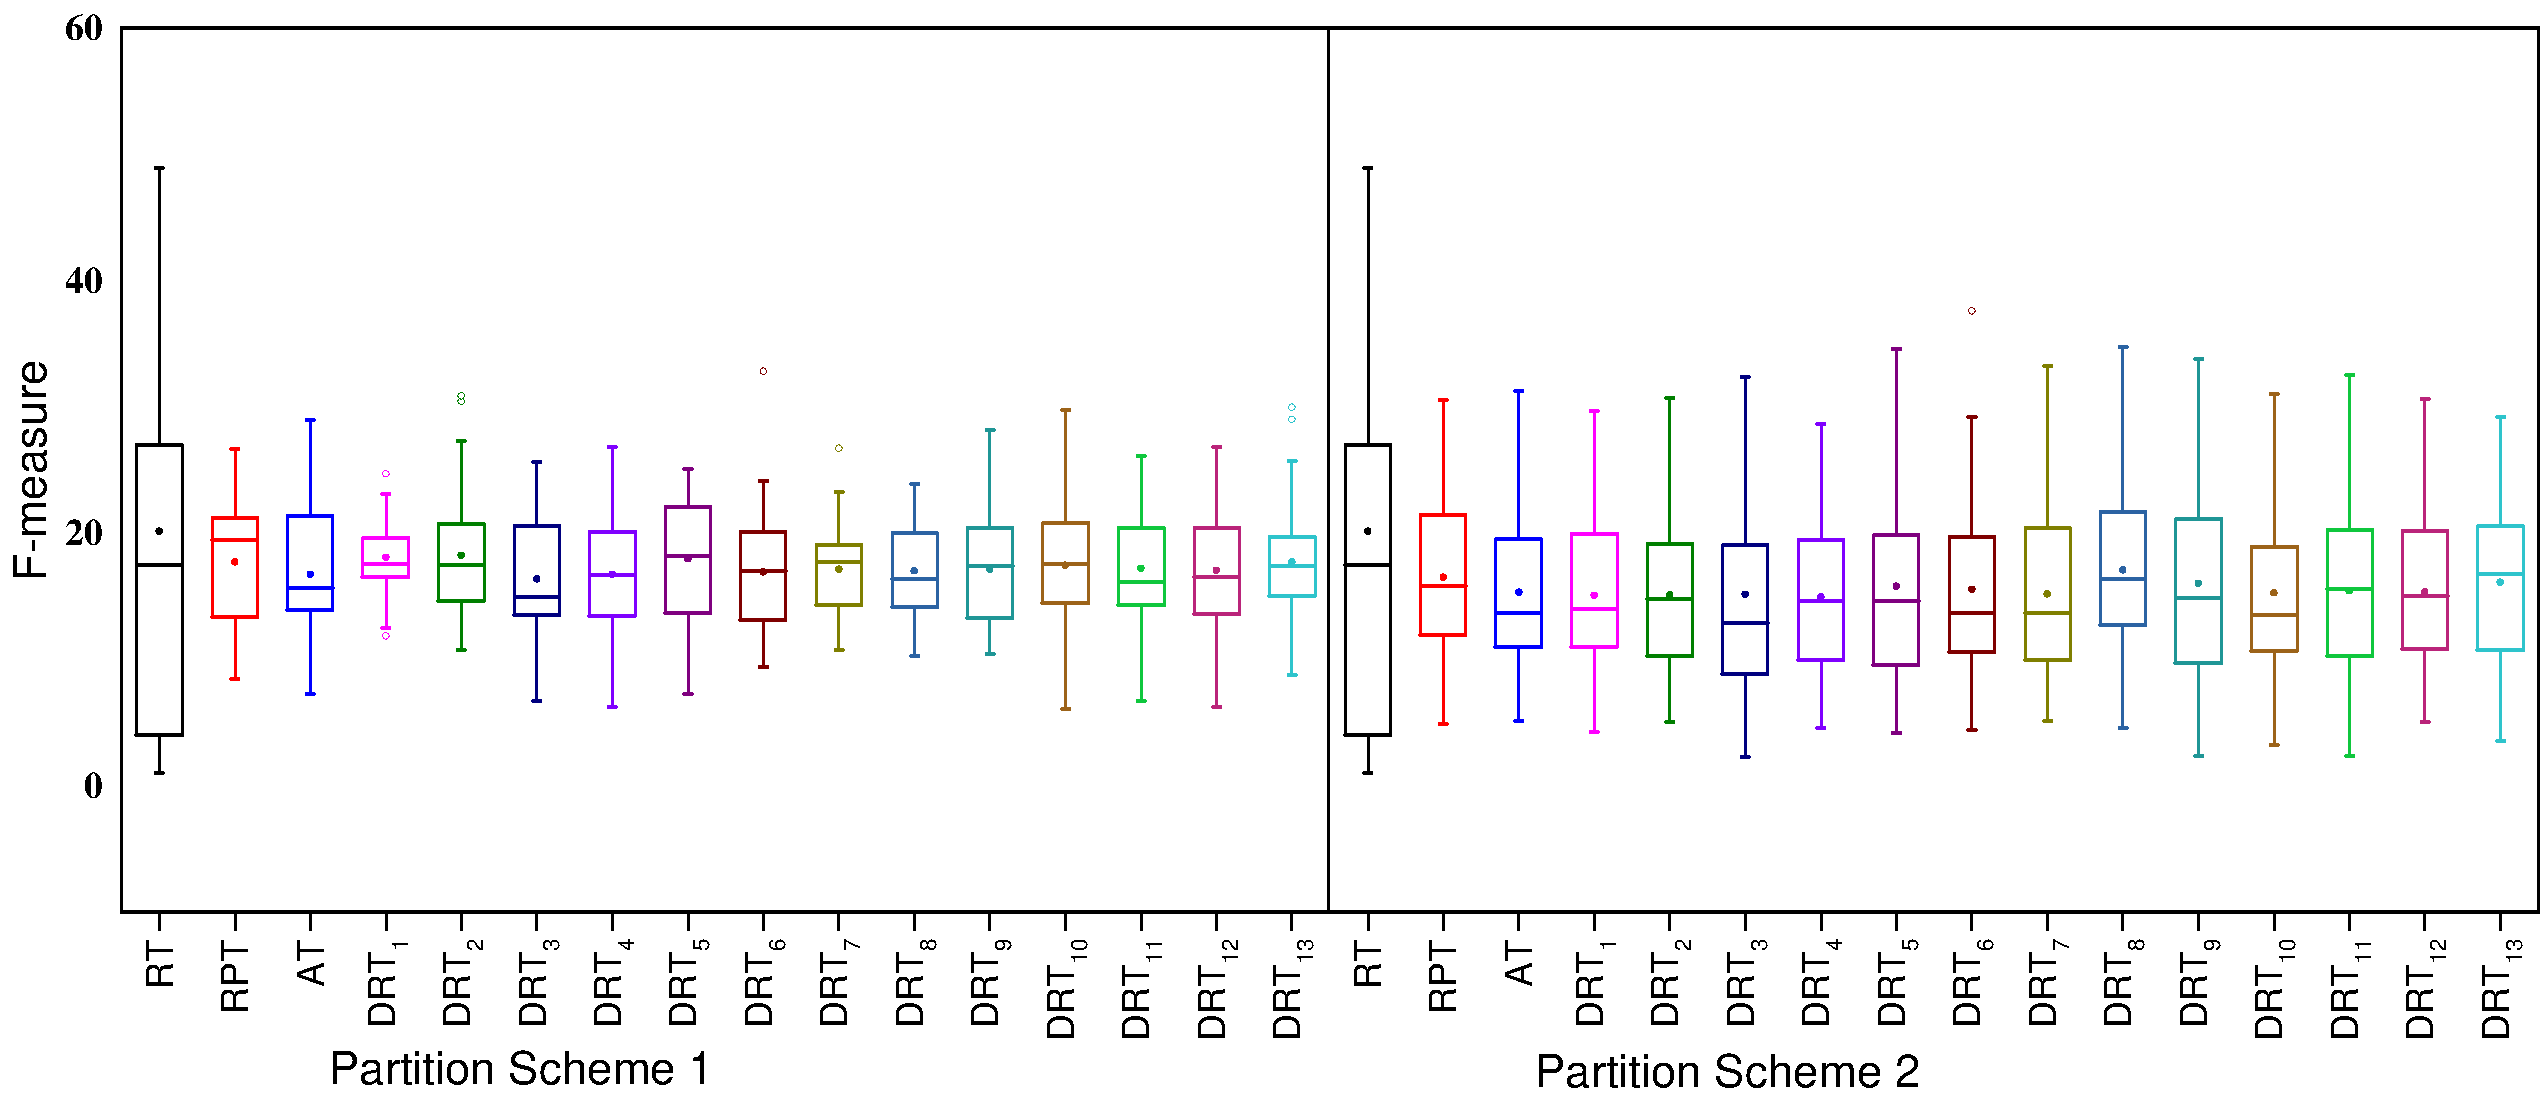
\includegraphics[width=0.9\textwidth,height=6.9cm]{fig/drtresultbox/parkingresultf.pdf}}
	\caption{F-measure boxplots for each web service}
	\label{fig:appendixFmeasure}
\end{figure*}

\begin{figure*}
	\centering
	\subfigure[ACMS] {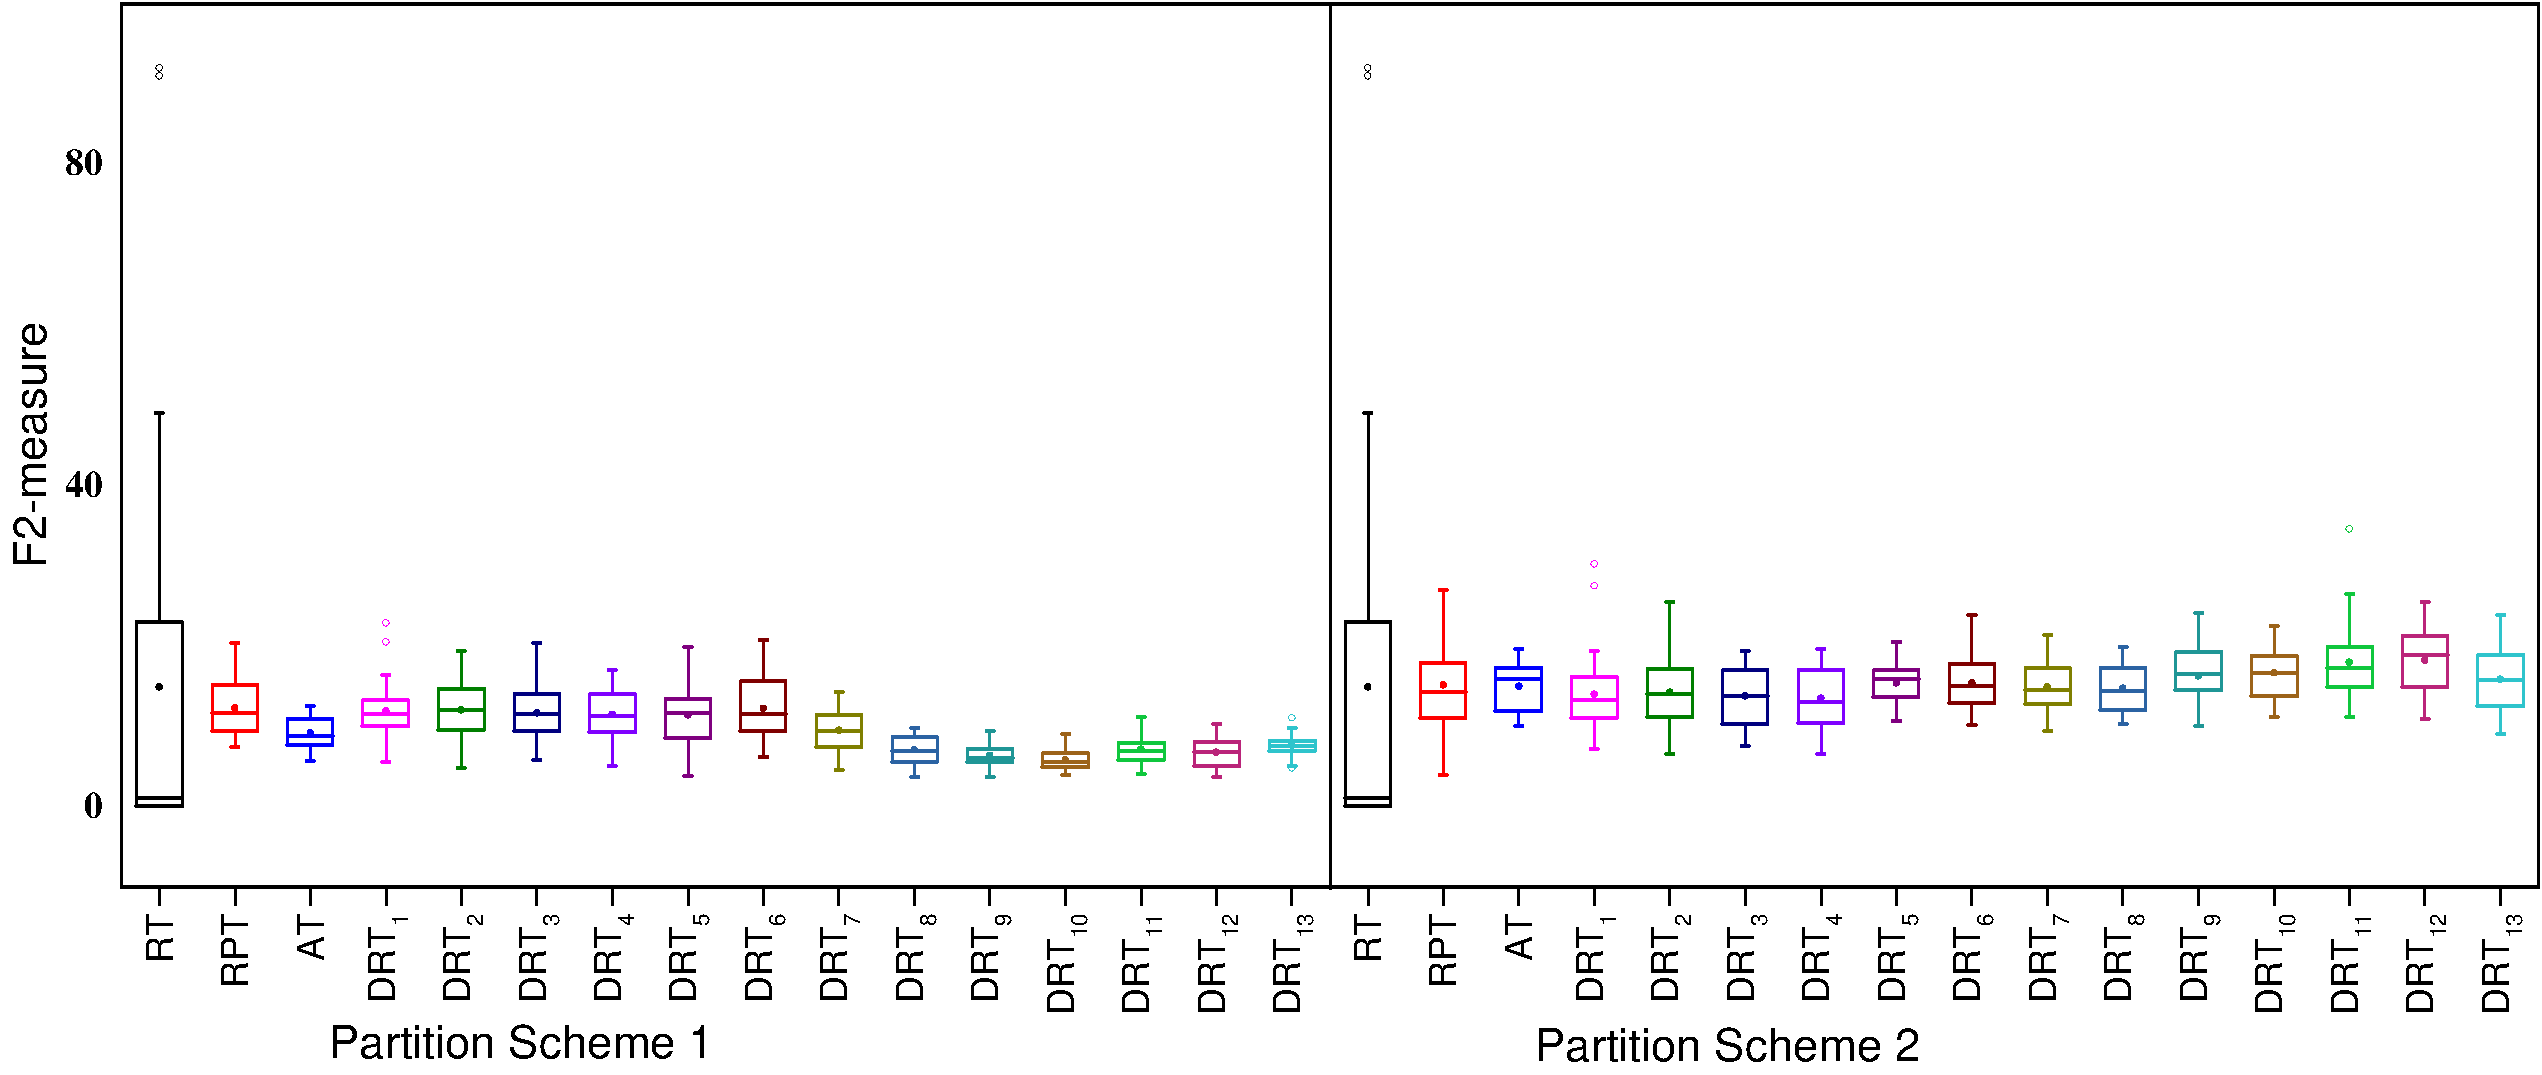
\includegraphics[width=0.9\textwidth,height=6cm]{fig/drtresultbox/aviaresultf2.pdf}}
	\subfigure[CUBS] {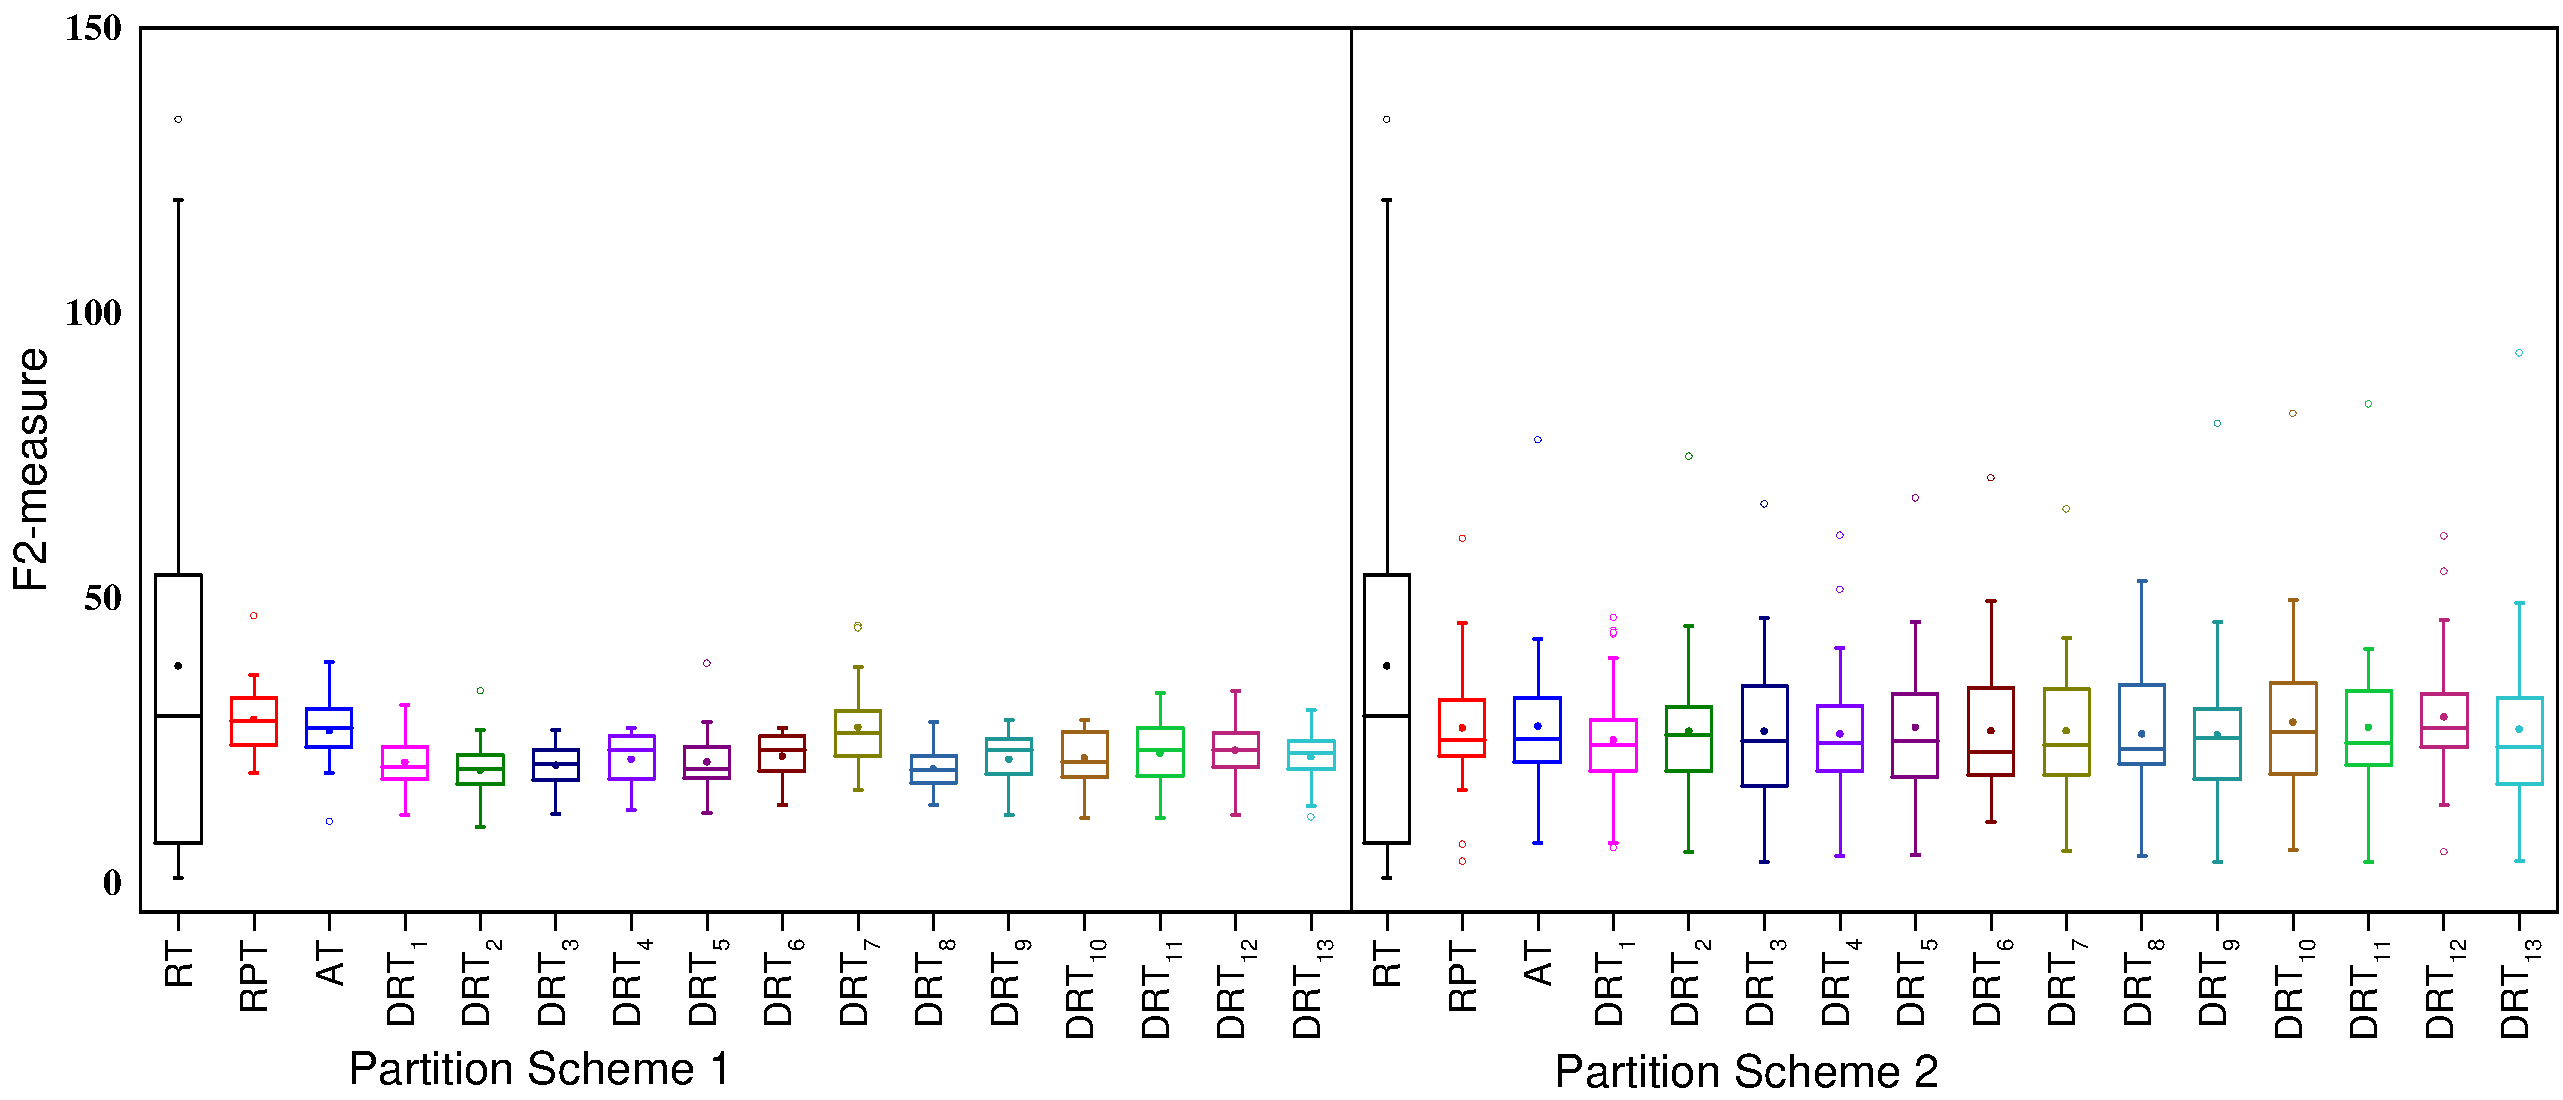
\includegraphics[width=0.9\textwidth,height=6cm]{fig/drtresultbox/chinaresultf2.pdf}}
	\subfigure[PBS] {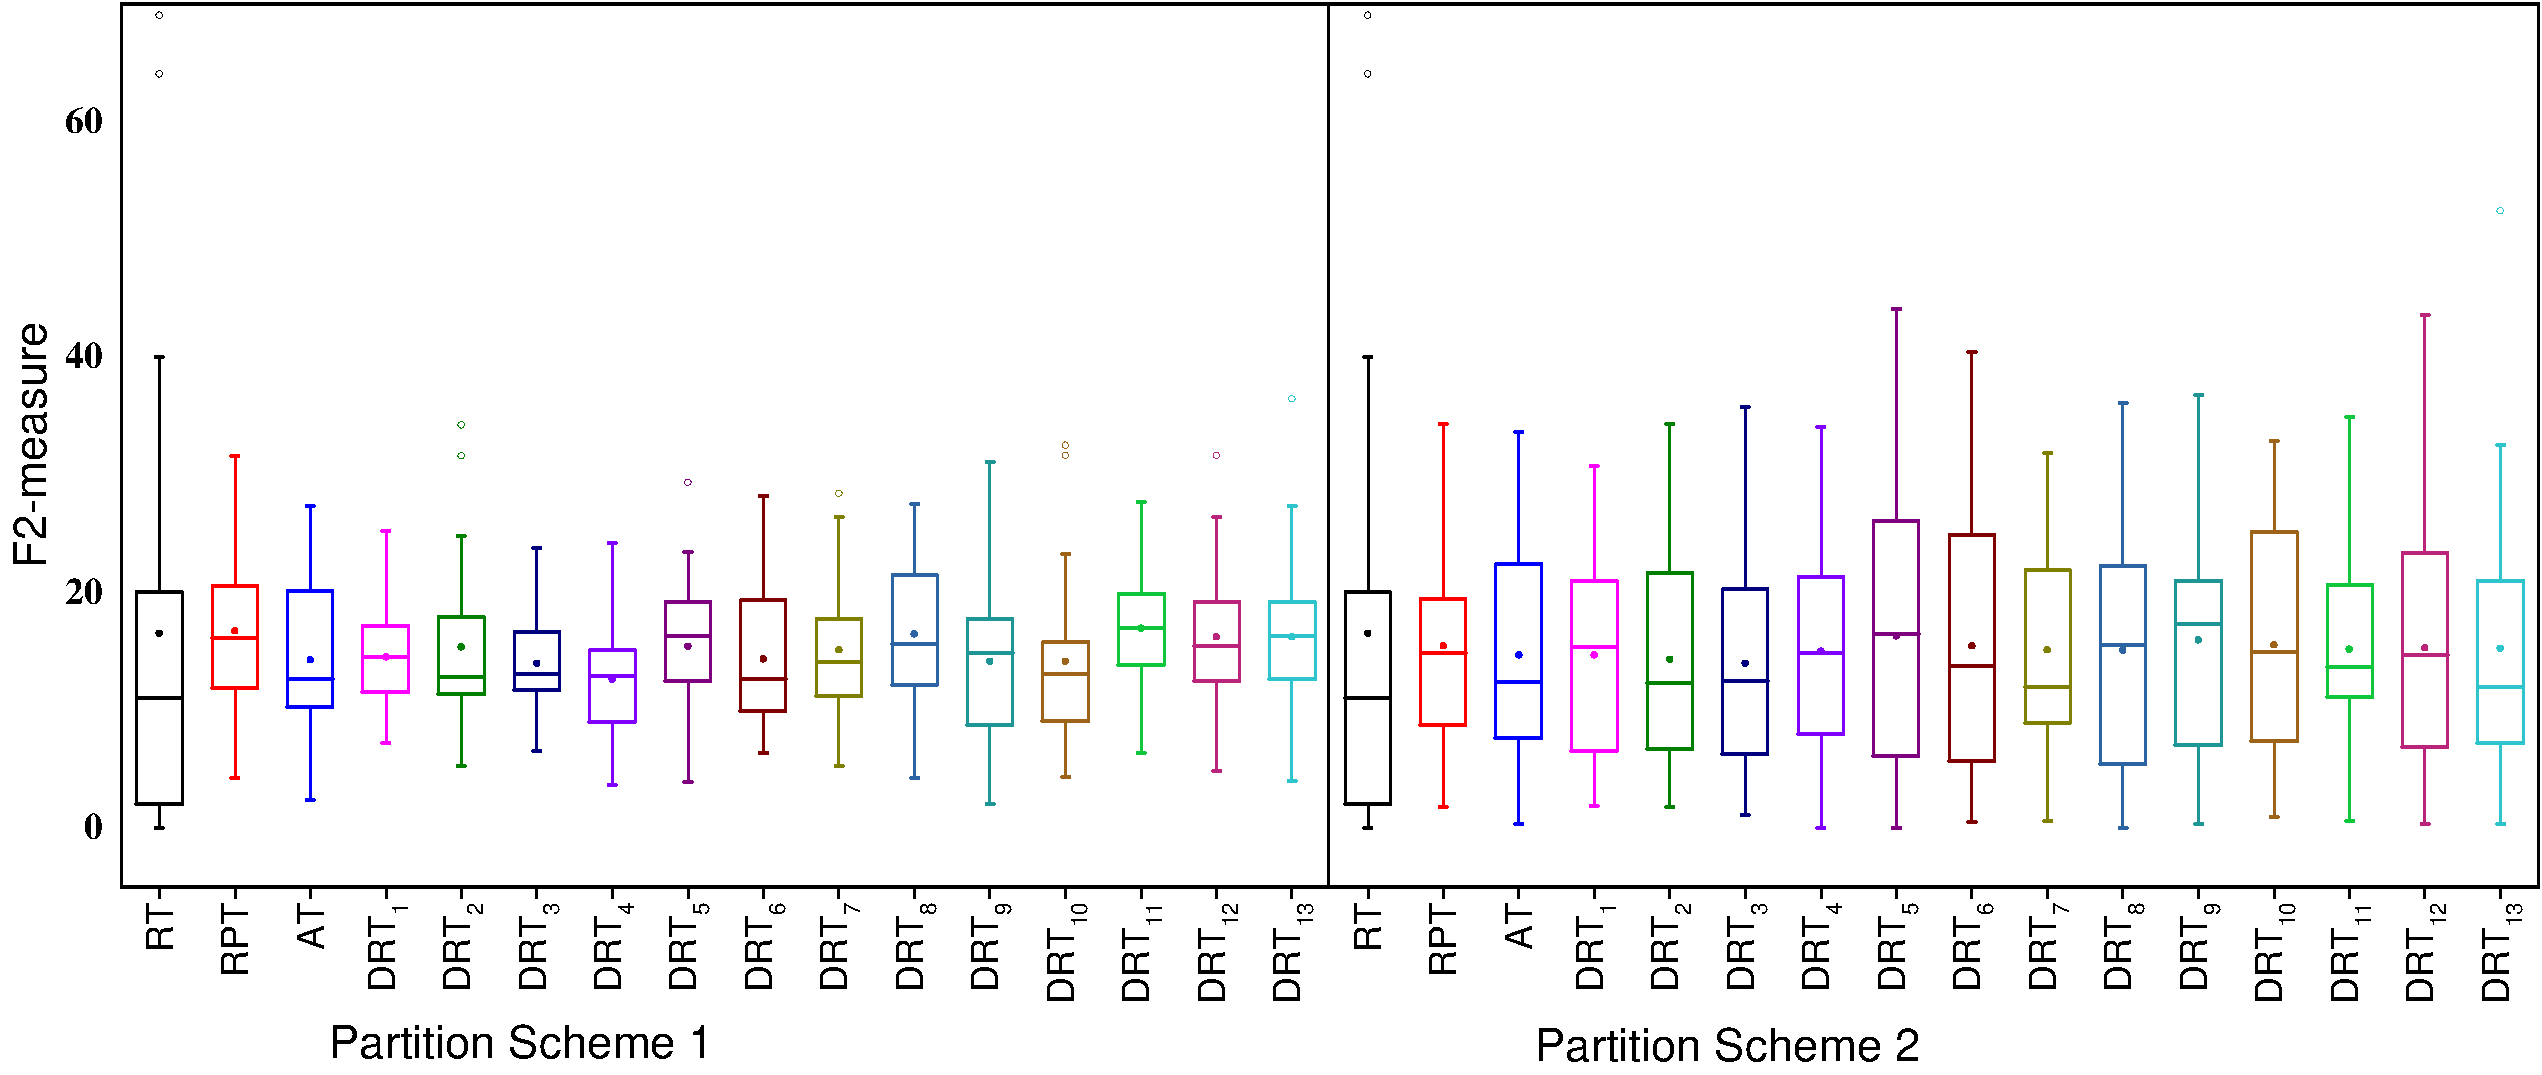
\includegraphics[width=0.9\textwidth,height=6cm]{fig/drtresultbox/parkingresultf2.pdf}}
	\caption{F2-measure boxplots for each web service}
	\label{fig:appendixF2measure}
\end{figure*}

\begin{figure*}
	\centering
	\subfigure[ACMS] {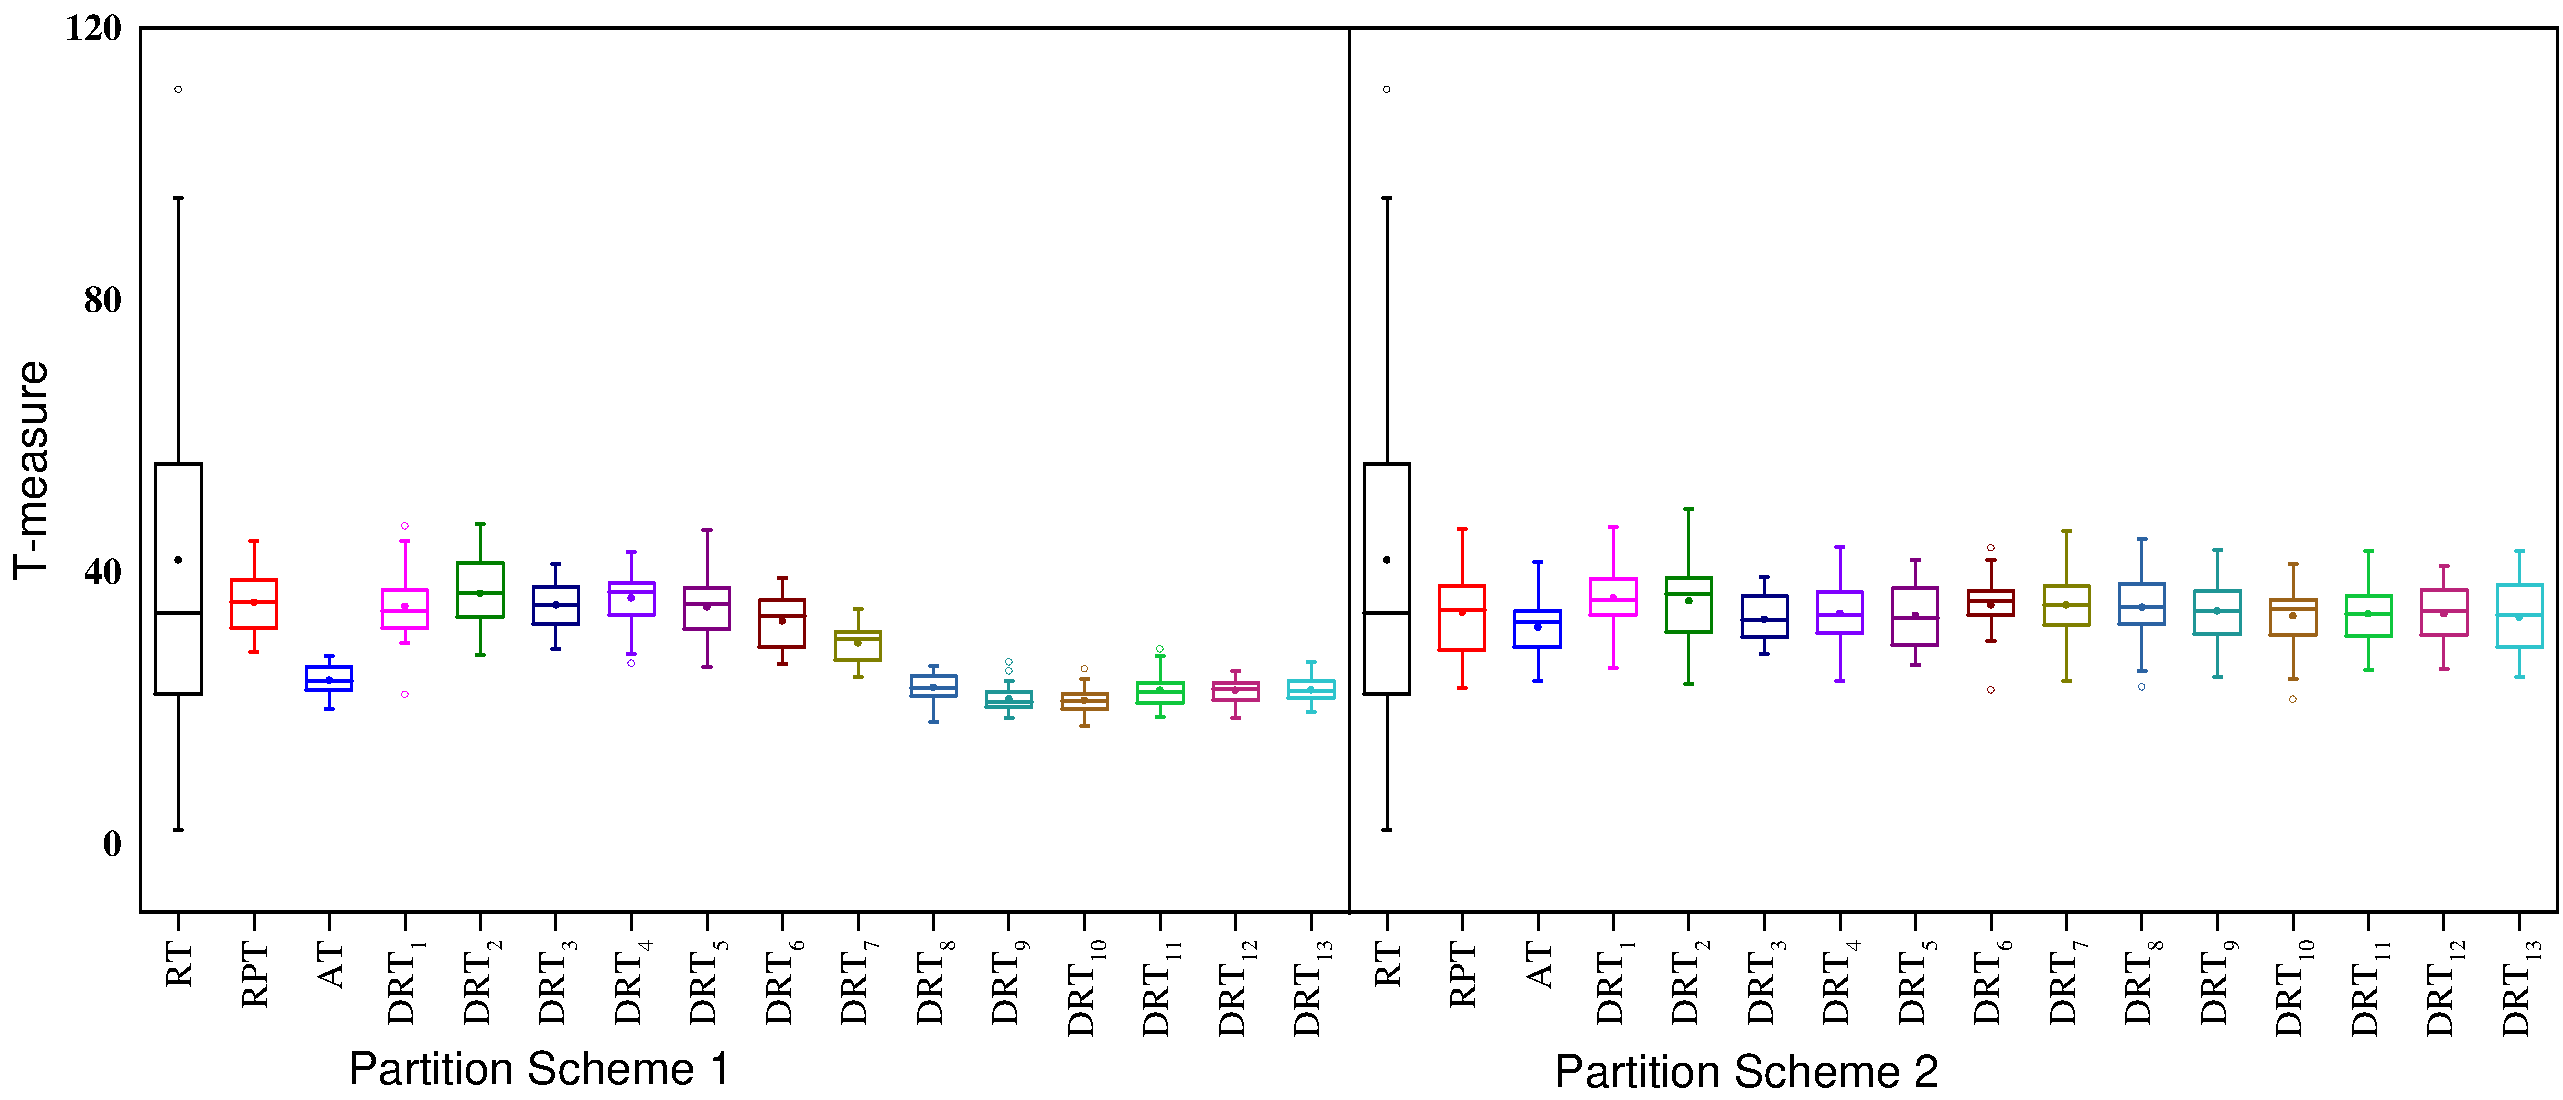
\includegraphics[width=0.9\textwidth,height=6cm]{fig/drtresultbox/aviaresultt.pdf}}
	\subfigure[CUBS] {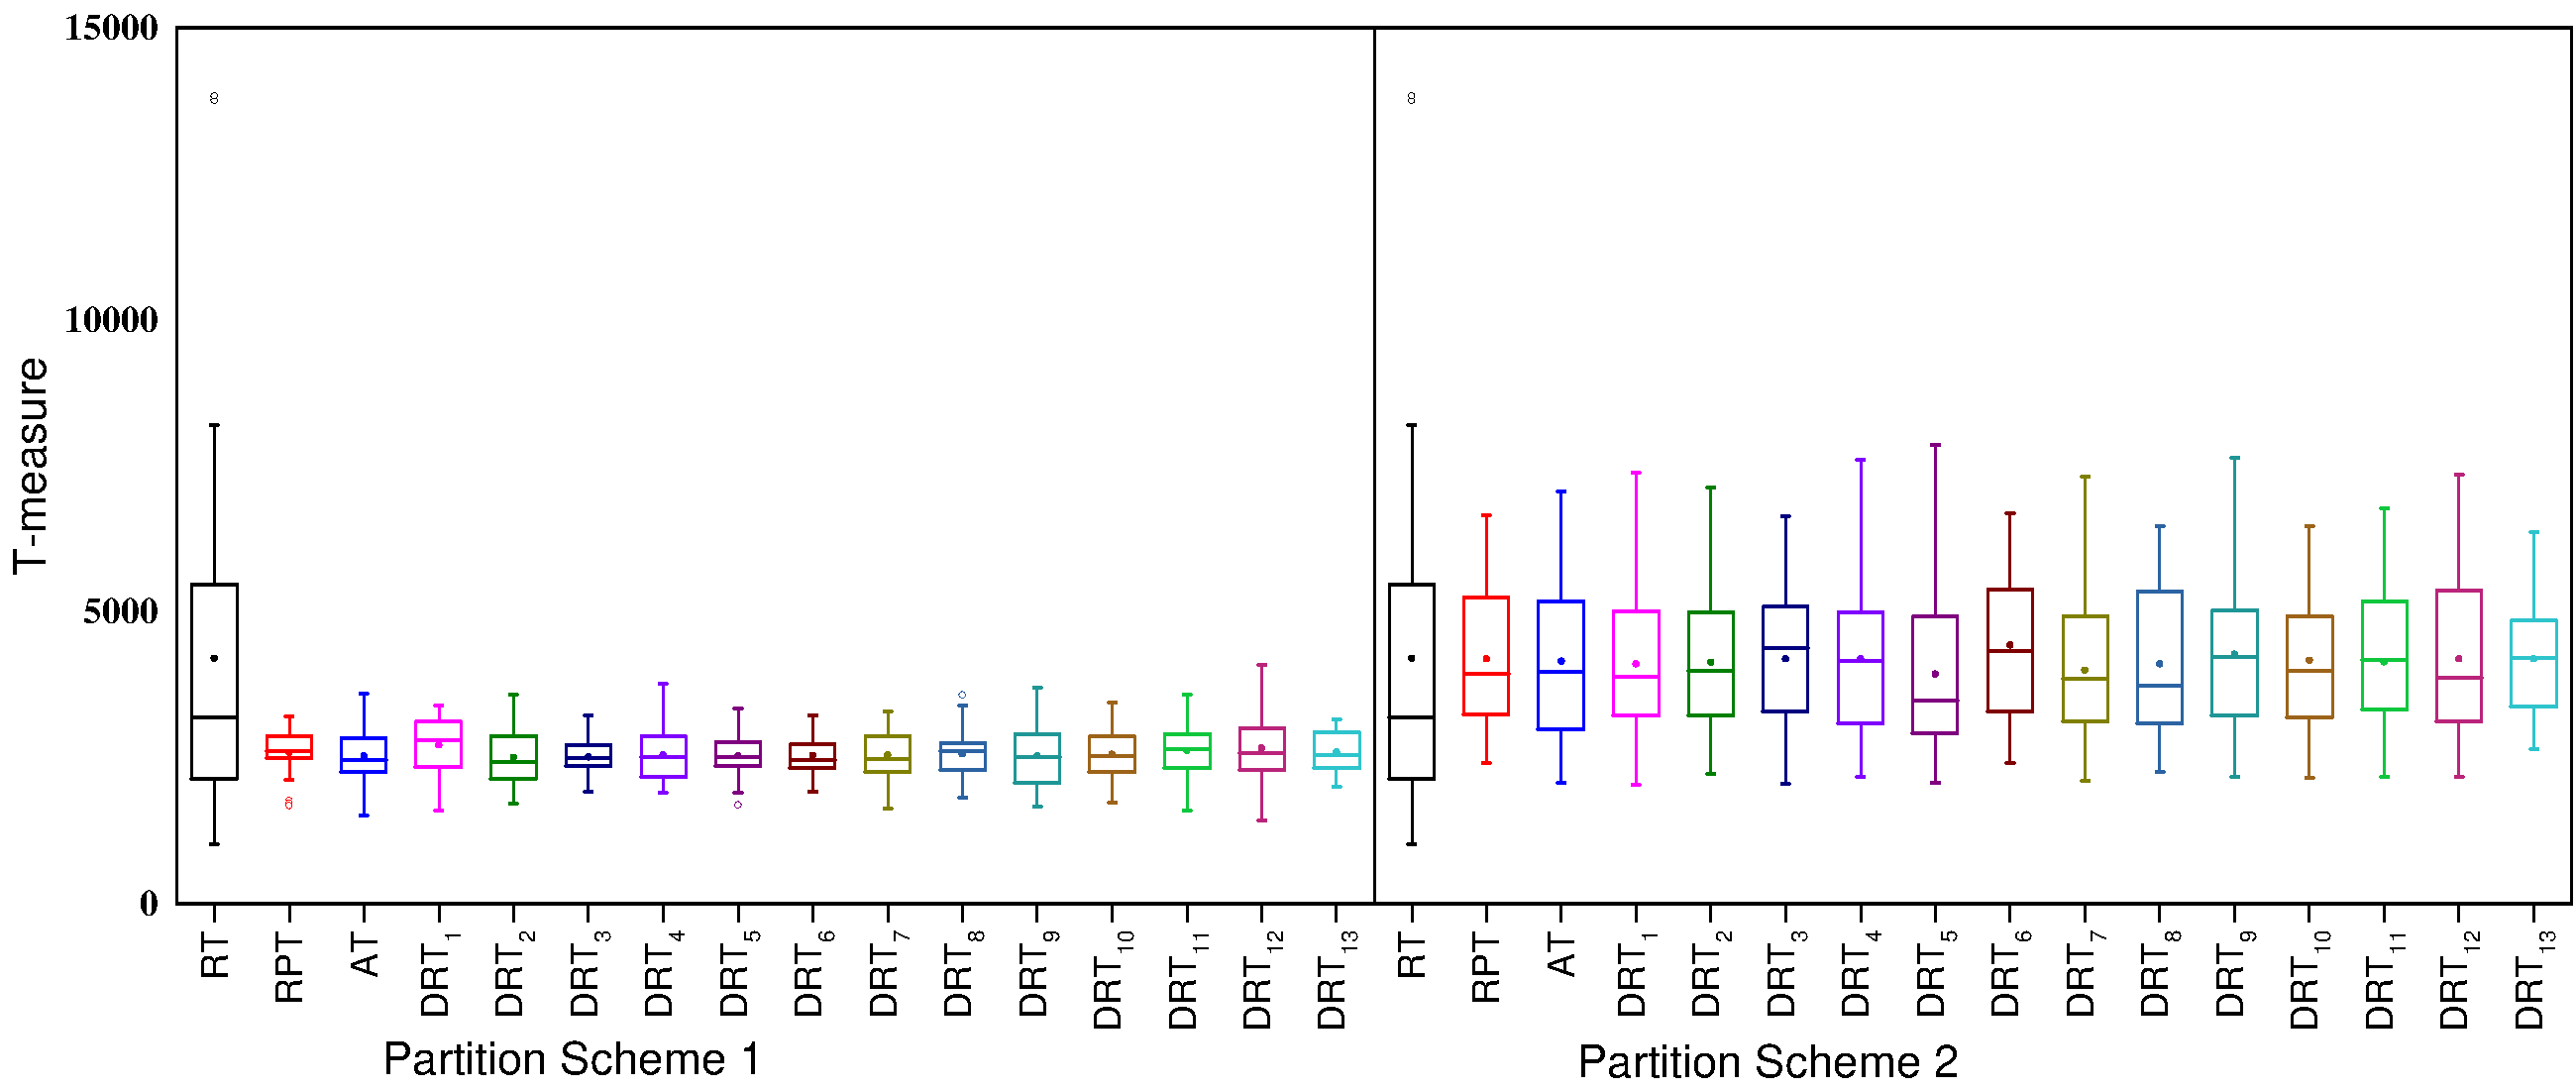
\includegraphics[width=0.9\textwidth,height=6cm]{fig/drtresultbox/chinaresultt.pdf}}
	\subfigure[PBS] {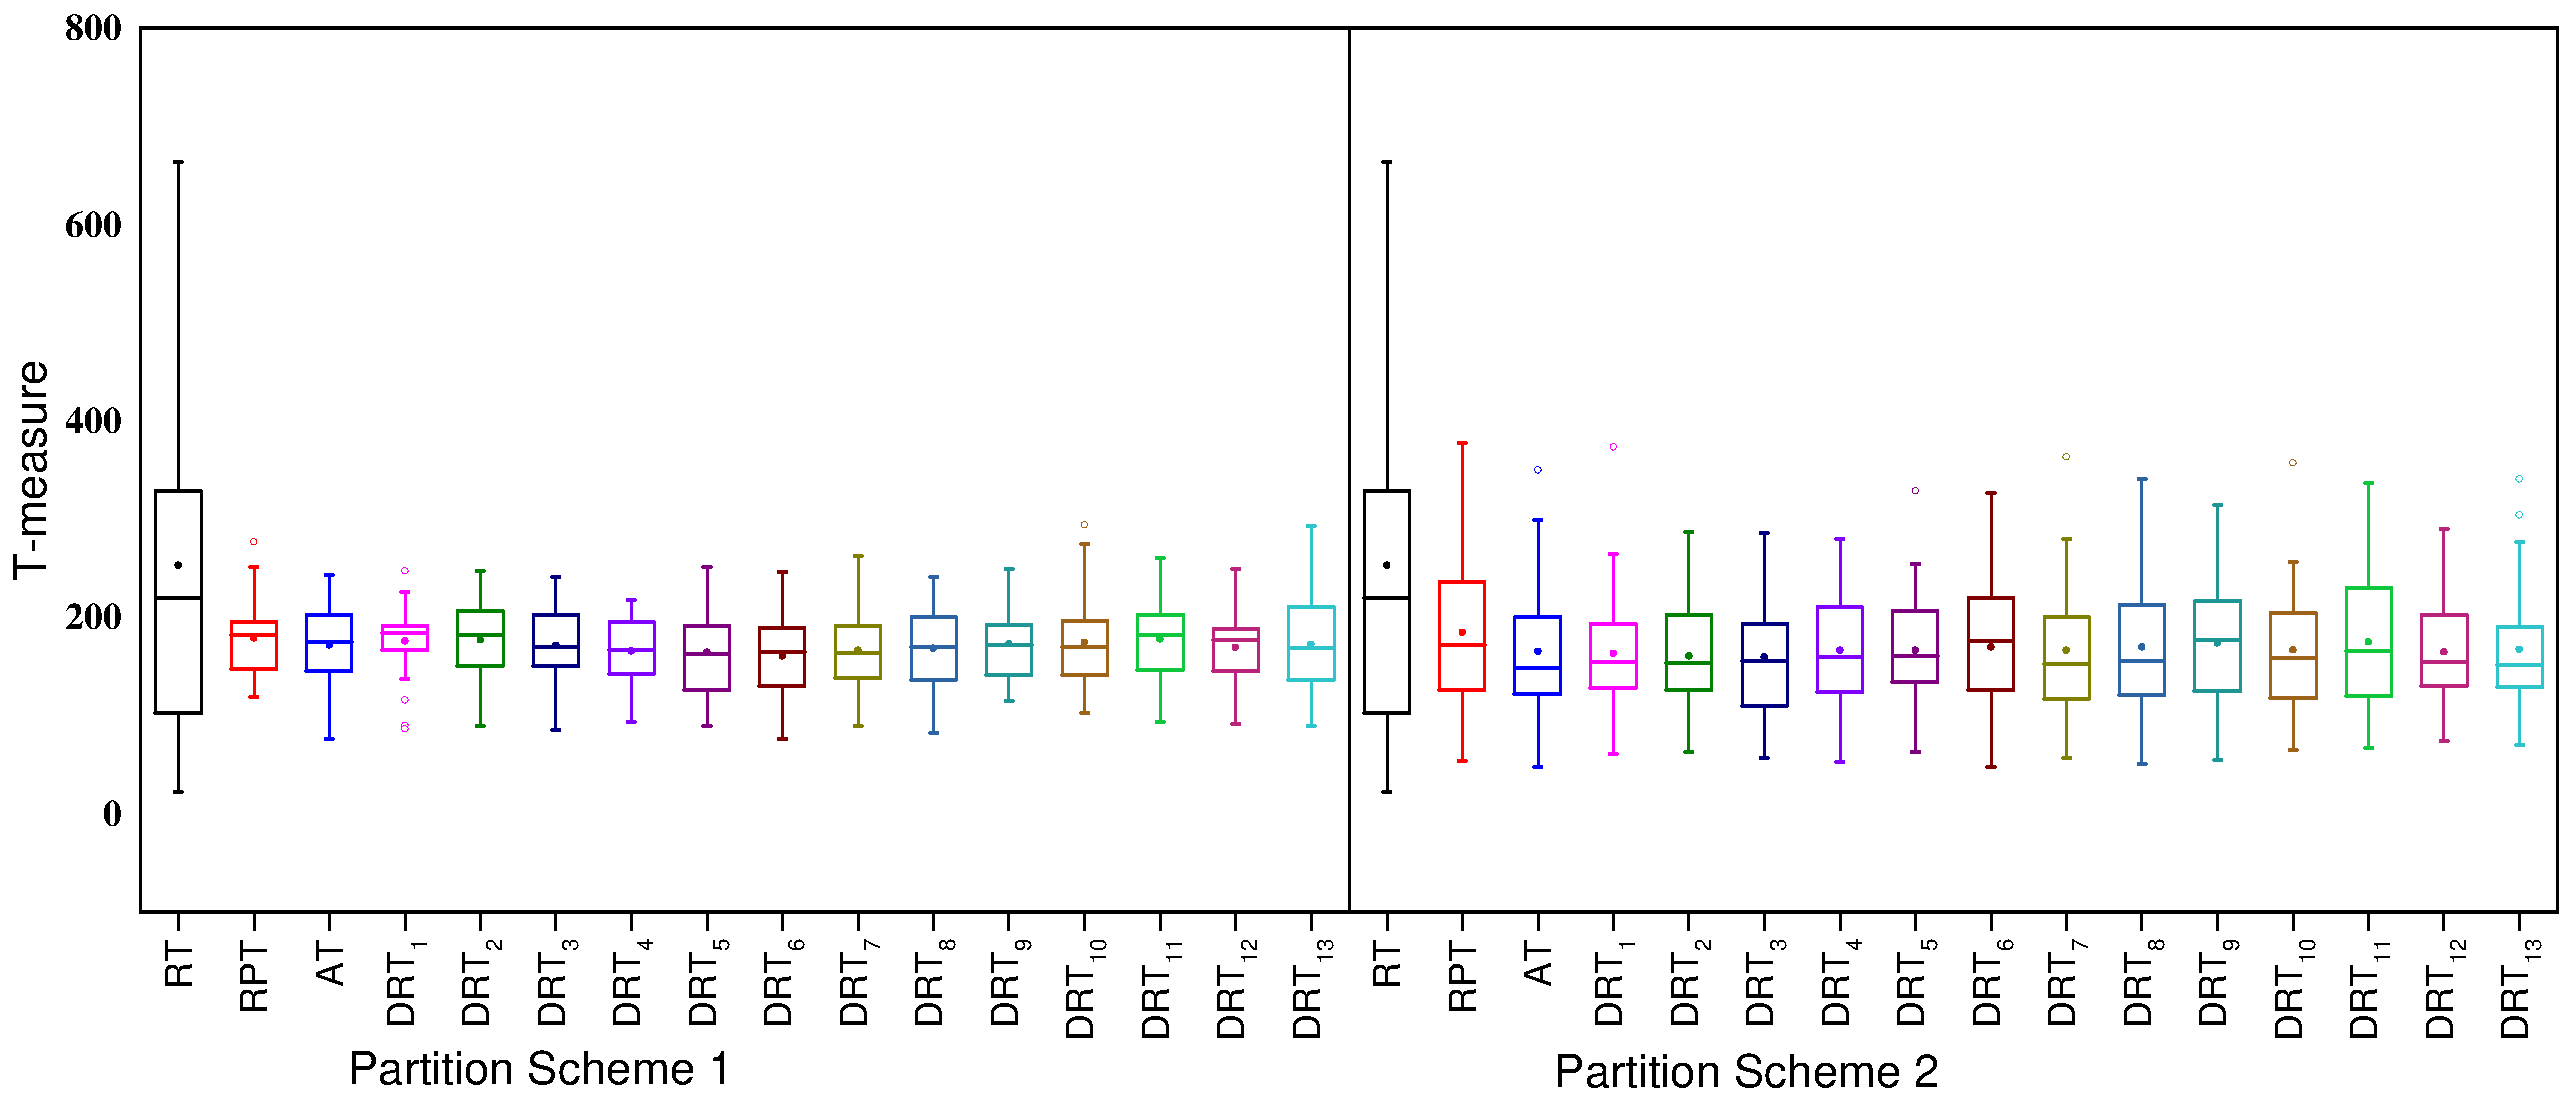
\includegraphics[width=0.9\textwidth,height=6cm]{fig/drtresultbox/parkingresultt.pdf}}
	\caption{T-measure boxplots for each web service}
	\label{fig:appendixTmeasure}
\end{figure*}


Tables \ref{tab:appendixtimeavia} to \ref{tab:appendixtimeparking} summarize the F-, F2-, and T-time results for three subject web services.

\begin{table}[h]
  \caption{F-time, F2-time and T-time for Web Service ACMS (in ms)}
  \label{tab:appendixtimeavia}
  \centering
  \setlength{\tabcolsep}{1mm}{
  \begin{tabular}{|c|c|c|c|c|c|c|c|} \hline
     \multicolumn{2}{|c|}{\multirow{2}{*}{Strategy}} &\multicolumn{3}{|c|}{Partition scheme 1} &\multicolumn{3}{|c|}{Partition scheme 2}\\ \cline{3-8}
     \multicolumn{2}{|c|}{}    &F-time	&F2-time &T-time &F-time &F2-time &T-time  \\ \hline
     \multicolumn{2}{|c|}{RT}  &0.43	&0.29	&0.85	&0.43 	&0.29	&0.85   \\ \hline
     \multicolumn{2}{|c|}{RPT} &0.57	&0.31	&1.08	&0.33	&0.45	&0.78   \\ \hline
     \multicolumn{2}{|c|}{AT}  &0.49    &0.34   &2.47   &15.53  &363.47 &459.67  \\ \hline
         \multirow{13}{*}{DRT} &1.0E-5    &0.47	&0.28	&0.96	&0.38	&0.41	&0.95  \\ \cline{2-8}
                               &5.0E-5	  &0.35	&0.21	&0.78	&0.30	&0.27	&0.71 \\ \cline{2-8}
                               &1.0E-4	  &0.33	&0.19	&0.66	&0.24	&0.28	&0.65 \\ \cline{2-8}
                               &5.0E-4	  &0.30	&0.17	&0.60	&0.27	&0.25	&0.67 \\ \cline{2-8}
                               &1.0E-3	  &0.29	&0.19	&0.61	&0.22	&0.24	&0.60 \\ \cline{2-8}
                               &5.0E-3	  &0.28	&0.23	&0.62	&0.21	&0.31	&0.64 \\ \cline{2-8}
                               &1.0E-2	  &0.24	&0.17	&0.53	&0.23	&0.29	&0.66 \\ \cline{2-8}
                               &5.0E-2	  &0.28	&0.13	&0.49	&0.23	&0.35	&0.71 \\ \cline{2-8}
                               &1.0E-1	  &0.26	&0.08	&0.43	&0.23	&0.29	&0.63 \\ \cline{2-8}
                               &2.0E-1	  &0.23	&0.12	&0.43	&0.30	&0.46	&0.89 \\ \cline{2-8}
                               &3.0E-1	  &0.24	&0.11	&0.45	&0.18	&0.40	&0.69 \\ \cline{2-8}
                               &4.0E-1	  &0.27	&0.10	&0.47	&0.16	&0.31	&0.58 \\ \cline{2-8}
                               &5.0E-1	  &0.28	&0.11	&0.47	&0.28	&0.45	&0.86 \\ \hline
  \end{tabular}}
\end{table}


\begin{table}[h]
  \caption{F-time, F2-time and T-time for Web Service CUBS (in ms)}
  \label{tab:appendixtimechina}
  \centering
  \setlength{\tabcolsep}{1mm}{
  \begin{tabular}{|c|c|c|c|c|c|c|c|} \hline
     \multicolumn{2}{|c|}{\multirow{2}{*}{Strategy}} &\multicolumn{3}{|c|}{Partition scheme 1} &\multicolumn{3}{|c|}{Partition scheme 2}\\ \cline{3-8}
     \multicolumn{2}{|c|}{}    &F-time	&F2-time &T-time &F-time &F2-time &T-time  \\ \hline
     \multicolumn{2}{|c|}{RT}  &0.82	&1.14	&34.69	&0.82	&1.14	&34.69   \\ \hline
     \multicolumn{2}{|c|}{RPT} &0.91	&0.87	&30.54	&0.75	&0.79	&34.59   \\ \hline
     \multicolumn{2}{|c|}{AT}  &140.13  &172.27 &32429.07 &16.82 &15.76 &2666.17 \\ \hline
         \multirow{13}{*}{DRT} &1.0E-5    &0.91	&0.87	&30.14	&0.87	&0.83	&36.49  \\ \cline{2-8}
                               &5.0E-5	  &0.95	&0.86	&30.21	&0.82	&0.75	&34.70\\ \cline{2-8}
                               &1.0E-4	  &0.77	&0.89	&29.27	&0.86	&0.69	&35.34 \\ \cline{2-8}
                               &5.0E-4	  &0.79	&1.00	&31.05	&0.87	&0.90	&36.85 \\ \cline{2-8}
                               &1.0E-3	  &0.86	&0.88	&29.93	&0.92	&0.77	&36.44 \\ \cline{2-8}
                               &5.0E-3	  &0.86	&0.83	&30.28	&0.83	&0.83	&36.27 \\ \cline{2-8}
                               &1.0E-2	  &0.95	&0.88	&29.33	&0.84	&0.72	&35.23 \\ \cline{2-8}
                               &5.0E-2	  &0.84	&0.82	&30.56	&0.88	&0.72	&37.07 \\ \cline{2-8}
                               &1.0E-1	  &0.88	&0.93	&29.45	&0.82	&0.76	&37.14 \\ \cline{2-8}
                               &2.0E-1	  &0.83	&0.83	&30.16	&0.86	&0.73	&36.79 \\ \cline{2-8}
                               &3.0E-1	  &0.95	&0.86	&27.81	&0.84	&0.84	&36.89 \\ \cline{2-8}
                               &4.0E-1	  &0.84	&0.84	&28.23	&0.86	&0.82	&35.22 \\ \cline{2-8}
                               &5.0E-1	  &0.87	&0.84	&27.91	&0.90	&0.86	&38.21 \\ \hline
  \end{tabular}}
\end{table}

\begin{table}[h]
  \caption{F-time, F2-time and T-time for Web Service PBS (in ms)}
  \label{tab:appendixtimeparking}
  \centering
  \setlength{\tabcolsep}{1mm}{
  \begin{tabular}{|c|c|c|c|c|c|c|c|} \hline
     \multicolumn{2}{|c|}{\multirow{2}{*}{Strategy}} &\multicolumn{3}{|c|}{Partition scheme 1} &\multicolumn{3}{|c|}{Partition scheme 2}\\ \cline{3-8}
     \multicolumn{2}{|c|}{}    &F-time	&F2-time &T-time &F-time &F2-time &T-time  \\ \hline
     \multicolumn{2}{|c|}{RT}  &0.81	&0.42	&4.12	&0.81	&0.42	&4.12   \\ \hline
     \multicolumn{2}{|c|}{RPT} &0.85	&0.52	&3.83	&0.66	&0.35	&2.98   \\ \hline
     \multicolumn{2}{|c|}{AT}  &22.25   &25.40  &289.04 &12.99  &17.44  &200.54 \\ \hline
         \multirow{13}{*}{DRT} &1.0E-5    &0.76	&0.48	&3.85	&1.05	&0.51	&3.44  \\ \cline{2-8}
                               &5.0E-5    &0.73	&0.35	&3.02	&0.91	&0.52	&3.79\\ \cline{2-8}
                               &1.0E-4    &0.54	&0.36	&2.97	&0.49	&0.34	&2.26 \\ \cline{2-8}
                               &5.0E-4    &0.68	&0.34	&3.20	&0.50	&0.30	&2.31 \\ \cline{2-8}
                               &1.0E-3    &0.62	&0.38	&2.87	&0.52	&0.38	&2.42 \\ \cline{2-8}
                               &5.0E-3    &0.60	&0.38	&2.99	&0.43	&0.51	&2.40 \\ \cline{2-8}
                               &1.0E-2    &0.58	&0.42	&2.84	&0.51	&0.34	&2.41 \\ \cline{2-8}
                               &5.0E-2    &0.64	&0.44	&3.27	&0.59	&0.36	&2.49 \\ \cline{2-8}
                               &1.0E-1    &0.65	&0.38	&3.46	&0.60	&0.38	&2.56 \\ \cline{2-8}
                               &2.0E-1	  &0.60	&0.36	&3.22	&0.54	&0.59	&2.47 \\ \cline{2-8}
                               &3.0E-1	  &0.59	&0.44	&3.24	&0.57	&0.46	&2.57 \\ \cline{2-8}
                               &4.0E-1	  &0.61	&0.33	&2.90	&0.51	&0.33	&2.54 \\ \cline{2-8}
                               &5.0E-1	  &0.62	&0.44	&3.16	&0.56	&0.36	&2.56 \\ \hline
  \end{tabular}}
\end{table}

\end{document}


